%%%%%%%%%%%%%%%%%%%%%%%%%%%%%%%%%%%%%%%%%
% Wenneker Assignment
% LaTeX Template
% Version 2.0 (12/1/2019)
%
% This template originates from:
% http://www.LaTeXTemplates.com
%
% Authors:
% Vel (vel@LaTeXTemplates.com)
% Frits Wenneker
%
% License:
% CC BY-NC-SA 3.0 (http://creativecommons.org/licenses/by-nc-sa/3.0/)
%
%%%%%%%%%%%%%%%%%%%%%%%%%%%%%%%%%%%%%%%%%

%----------------------------------------------------------------------------------------
%	PACKAGES AND OTHER DOCUMENT CONFIGURATIONS
%----------------------------------------------------------------------------------------

\documentclass[11pt]{scrartcl} % Font size
\usepackage{comment}
\usepackage{color}
%%%%%%%%%%%%%%%%%%%%%%%%%%%%%%%%%%%%%%%%%
% Wenneker Assignment
% Structure Specification File
% Version 2.0 (12/1/2019)
%
% This template originates from:
% http://www.LaTeXTemplates.com
%
% Authors:
% Vel (vel@LaTeXTemplates.com)
% Frits Wenneker
%
% License:
% CC BY-NC-SA 3.0 (http://creativecommons.org/licenses/by-nc-sa/3.0/)
% 
%%%%%%%%%%%%%%%%%%%%%%%%%%%%%%%%%%%%%%%%%

%----------------------------------------------------------------------------------------
%	PACKAGES AND OTHER DOCUMENT CONFIGURATIONS
%----------------------------------------------------------------------------------------

\usepackage{amsmath, amsfonts, amsthm} % Math packages
\usepackage{tabto}
\usepackage{listings} % Code listings, with syntax highlighting
\usepackage{tabu}
\usepackage{array}
\usepackage[english]{babel} % English language hyphenation
\usepackage{hyperref}

\usepackage{graphicx} % Required for inserting images
\graphicspath{{Figures/}{./}} % Specifies where to look for included images (trailing slash required)

\usepackage{booktabs} % Required for better horizontal rules in tables

\numberwithin{equation}{section} % Number equations within sections (i.e. 1.1, 1.2, 2.1, 2.2 instead of 1, 2, 3, 4)
\numberwithin{figure}{section} % Number figures within sections (i.e. 1.1, 1.2, 2.1, 2.2 instead of 1, 2, 3, 4)
\numberwithin{table}{section} % Number tables within sections (i.e. 1.1, 1.2, 2.1, 2.2 instead of 1, 2, 3, 4)

\setlength\parindent{0pt} % Removes all indentation from paragraphs

\usepackage{enumitem} % Required for list customisation
\setlist{noitemsep} % No spacing between list items

%----------------------------------------------------------------------------------------
%	DOCUMENT MARGINS
%----------------------------------------------------------------------------------------

\usepackage{geometry} % Required for adjusting page dimensions and margins

\geometry{
	paper=a4paper, % Paper size, change to letterpaper for US letter size
	top=2.5cm, % Top margin
	bottom=3cm, % Bottom margin
	left=3cm, % Left margin
	right=3cm, % Right margin
	headheight=0.75cm, % Header height
	footskip=1.5cm, % Space from the bottom margin to the baseline of the footer
	headsep=0.75cm, % Space from the top margin to the baseline of the header
	%showframe, % Uncomment to show how the type block is set on the page
}

%----------------------------------------------------------------------------------------
%	FONTS
%----------------------------------------------------------------------------------------

\usepackage[utf8]{inputenc} % Required for inputting international characters
\usepackage[T1]{fontenc} % Use 8-bit encoding

\usepackage{fourier} % Use the Adobe Utopia font for the document

%----------------------------------------------------------------------------------------
%	SECTION TITLES
%----------------------------------------------------------------------------------------

\usepackage{sectsty} % Allows customising section commands

\sectionfont{\vspace{6pt}\centering\normalfont\scshape} % \section{} styling
\subsectionfont{\normalfont\bfseries} % \subsection{} styling
\subsubsectionfont{\normalfont\itshape} % \subsubsection{} styling
\paragraphfont{\normalfont\scshape} % \paragraph{} styling

%----------------------------------------------------------------------------------------
%	HEADERS AND FOOTERS
%----------------------------------------------------------------------------------------

\usepackage{scrlayer-scrpage} % Required for customising headers and footers

\ohead*{} % Right header
\ihead*{} % Left header
\chead*{} % Centre header

\ofoot*{} % Right footer
\ifoot*{} % Left footer
\cfoot*{\pagemark} % Centre footer
 % Include the file specifying the document structure and custom commands
\usepackage{graphicx}
\usepackage{subcaption}



%Code retrieved from: https://www.overleaf.com/project/5c52d66b6343590b46b4fd03


%----------------------------------------------------------------------------------------
%	TITLE SECTION
%----------------------------------------------------------------------------------------

\title{
	\normalfont\normalsize
	\textsc{Old Dominion University}\\ % Your university, school and/or department name(s)
	\vspace{25pt} % Whitespace
	\rule{\linewidth}{0.5pt}\\ % Thin top horizontal rule
	\vspace{20pt} % Whitespace
	{\huge Assignment 4}\\ % The assignment title
	\vspace{12pt} % Whitespace
	\rule{\linewidth}{2pt}\\ % Thick bottom horizontal rule
	\vspace{12pt} % Whitespace
}

\author{\LARGE David Bayard} % Your name

\date{\normalsize\today} % Today's date (\today) or a custom date

\begin{document}

\definecolor{codegreen}{rgb}{0,0.6,0}
\definecolor{codegray}{rgb}{0.5,0.5,0.5}
\definecolor{codepurple}{rgb}{0.58,0,0.82}
\definecolor{backcolour}{rgb}{0.95,0.95,0.92}
\lstdefinestyle{pythonStyle}{
  backgroundcolor=\color{backcolour},
  commentstyle=\color{codegreen},
  keywordstyle=\color{magenta},
  numberstyle=\tiny\color{codegray},
  stringstyle=\color{codepurple},
  basicstyle=\footnotesize,
  breakatwhitespace=false,
  breaklines=true,
  captionpos=b,
  keepspaces=true,
  numbers=left,
  numbersep=5pt,
  showspaces=false,
  showstringspaces=false,
  showtabs=false,
  tabsize=2
}

\lstset{style=pythonStyle}


\maketitle % Print the title

\pagebreak
\section*{Question 1.}



%------------------------------------------------

\subsection*{Determine if the friendship paradox holds for my Facebook
account.}
\bigskip\bigskip


\LARGE Solution:
\newline \newline\small

\tabto{2.0cm} In order to determine if the friendship paradox is enforced, the mean, median, and standard deviation of professor Nwalas friends was calculated. This was done by reading the .csv file provided by professor Nwala and using built in python functions to calculate each data point, for example, the mean was calculated as shown:

\begin{lstlisting}[language = Python, caption=Calculating Mean]
  average = statistics.mean(listValues)
  roundedAverage = round(average,2)
\end{lstlisting} \bigskip 

\tabto{2.0cm} The code above displays using the Statistics library to calculate the mean, the same was done for the median and standard deviation. A simple counter was used to keep track of the number of friends that professor Nwala has. Once the mean, median, and friend count were calculated, it was evident that the friendship paradox does, in fact, hold. 
\newline \newline
\tabto{2.0cm} It is evident that the friendship paradox holds because professor Nwalas friend count is significantly smaller than the mean friend count. This means that professor Nwala has less friends then his friends have, on average. This point is illustrated on the graph below, which displays the distance between professor Nwalas friend count and the average friend count.
\begin{figure}[h!]
\begin{center}
\begin{subfigure}[b]{1.1\linewidth }
    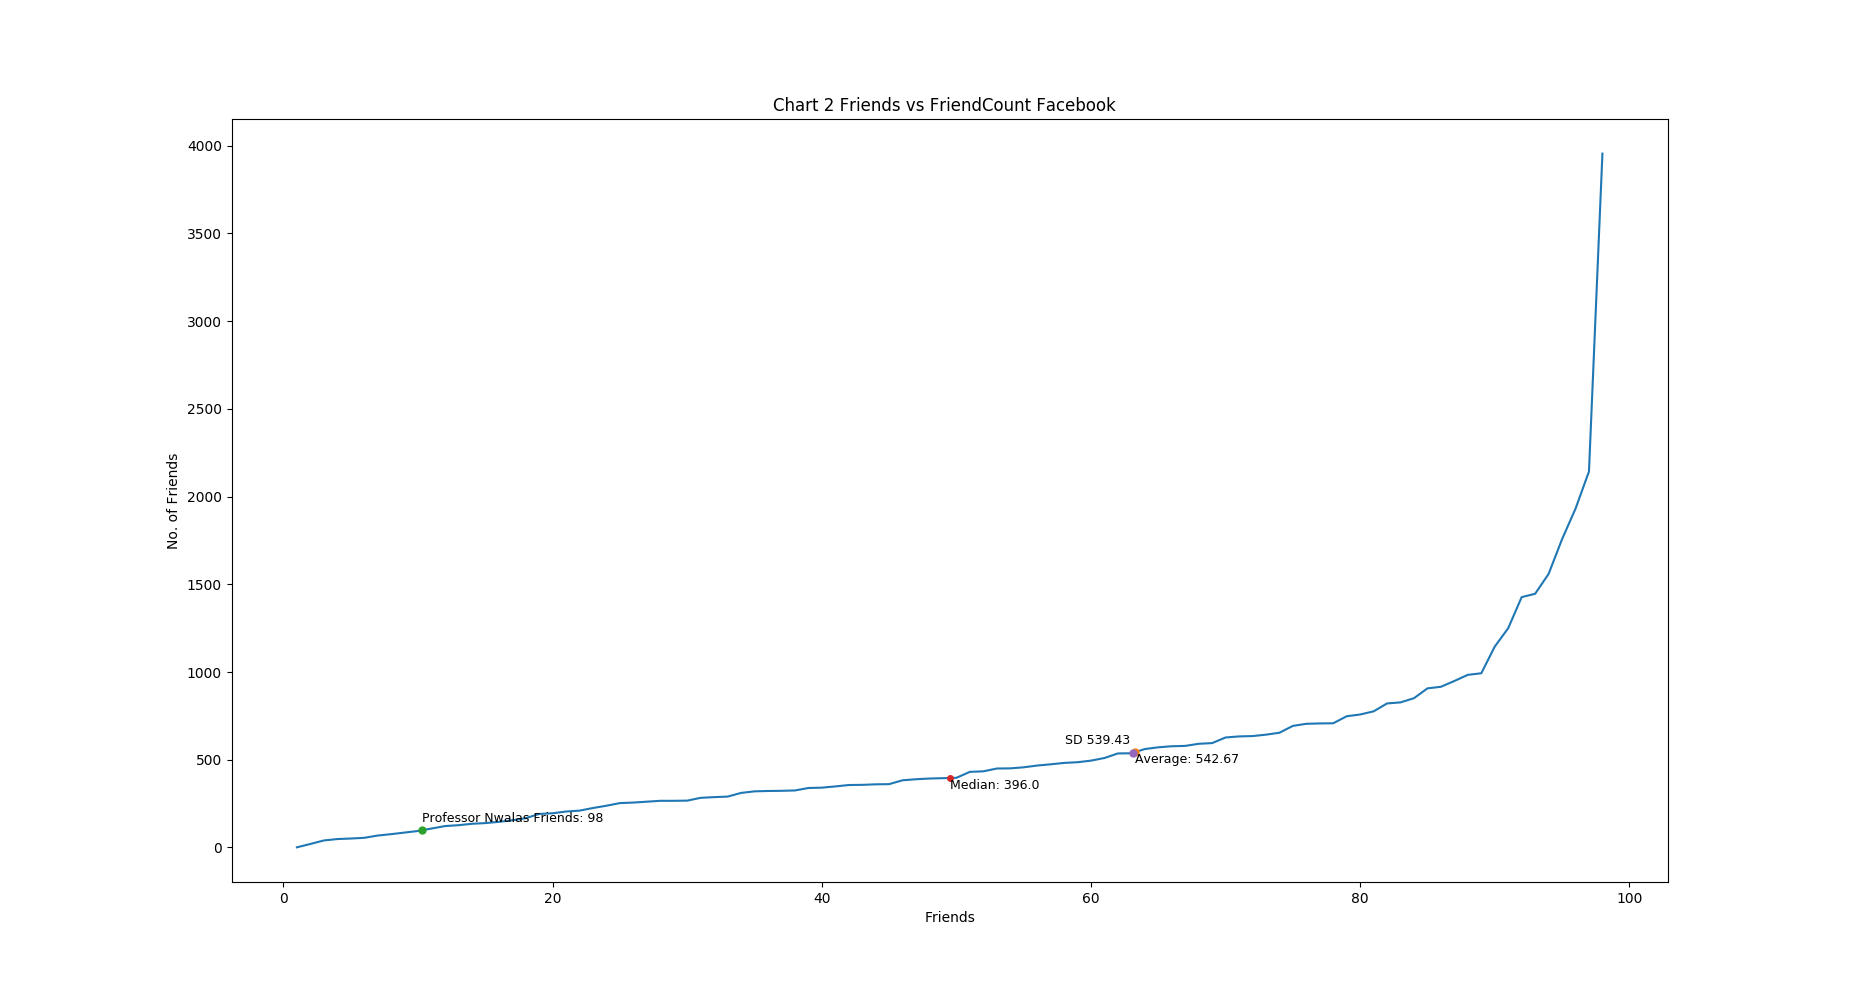
\includegraphics[width=\linewidth]{../Figures/FacebookGraph.png}
    \caption{Facebook Graph}
\end{subfigure}
\end{center}
\end{figure}

\pagebreak

\section*{Question 2}


\subsection*{Determine if the friendship paradox holds for your Twitter account.
Since Twitter is a directed graph, use "followers" as value you measure}

%------------------------------------------------
\bigskip\bigskip
\LARGE Solution: \newline\newline\small

\tabto{2.0cm} In order to determine if the friendship paradox holds for a Twitter account, the number of followers for each follower had to be captured. In this case, professor Nwalas Twitter handle ``acnwala'' was used, and the number of followers for each of his followers was extracted using the Tweepy API. The Tweepy API provides a method to search for followers, which returns User objects, providing each follower for that user, and their number of followers. The usage of this API is demonstrated below.

\begin{lstlisting}[language = Python, caption=Getting User Objects]
try:
        for user in tweepy.Cursor(api.followers, screen_name="acnwala").items():
            followers.append(user)
            counter += 1
\end{lstlisting} \bigskip 

\tabto{2.0cm} In the above code, the Tweepy API is used to extract User objects, and these objects are stored in the followers list. The counter variable keeps track of the total number of followers that professor Nwala has. Next, it is necessary to extract the number of followers that each follower has, and this is demonstrated below.


\begin{lstlisting}[language = Python, caption=Extracting Follower Count]
  for follower in followers:
    writer.writerow({'User': follower.name, 'FriendCount': follower.followers_count})
\end{lstlisting}

\tabto{2.0cm} As demonstrated above, each User object provides methods that can be used to extract the name of each follower, along with their follower count. With this information, we can calculate the mean, median, and standard deviation of each of the followers just as was done from question 1. The graph below illustrates the information that was gathered from Twitter.

\begin{figure}[h!]
\begin{subfigure}[b]{1.0\linewidth }
    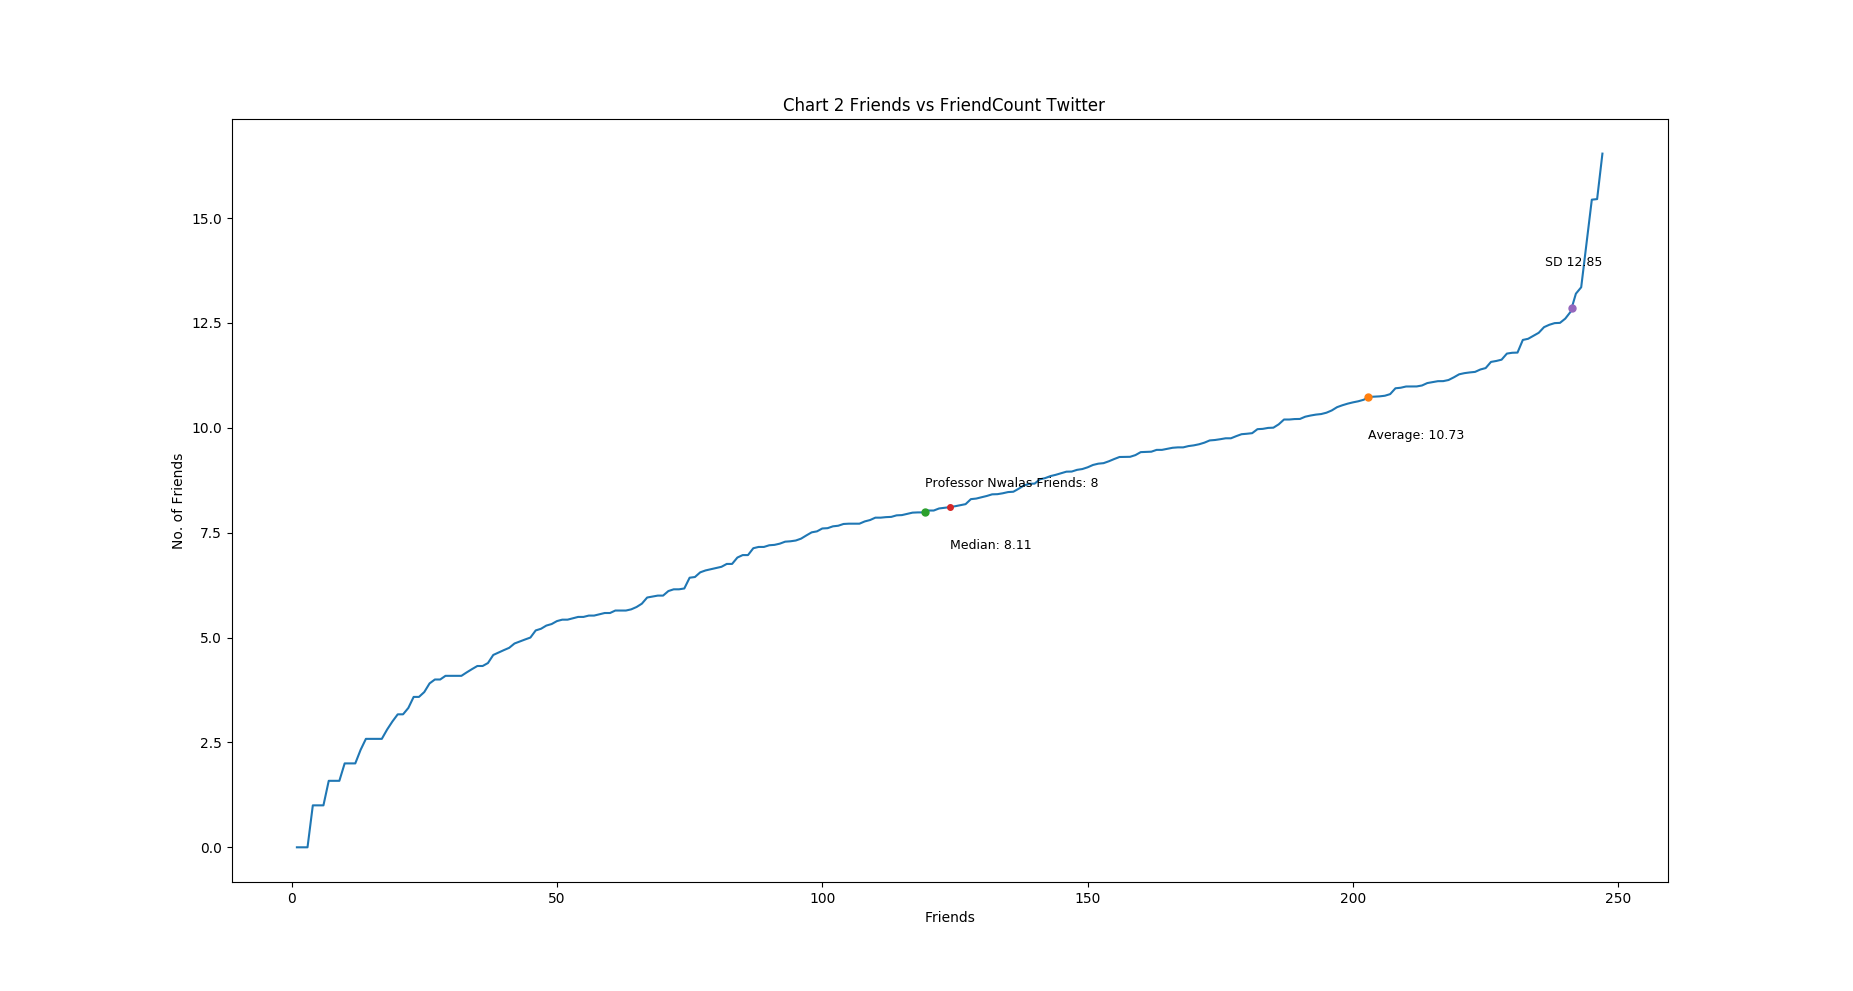
\includegraphics[width=\linewidth]{../Figures/TwitterGraph.png}
    \caption{Twitter Graph}
\end{subfigure}
\end{figure}

\tabto{2.0 cm}The figure in page 2 was created using a logarithmic function with a base of 2, for each of the y values. This was done because there were several outliers, ranging from 0 to 90000 friends. This severely skewed the graph, and using a logarithmic function reduced this skew and demonstrates an accurate representation of the data. 
\newline \newline

\tabto{2.0cm} The values for the mean, median, standard deviation, and personal count before the logarithmic function was supplied are listed below.
\bigskip \bigskip
\begin{center}
\begin{LARGE} Statistics Before Logarithmic Function  \end{LARGE} \newline \newline
\begin{tabular}{ |p{1cm}||p{1cm}|p{6cm}|p{6cm}|  }
 \hline
 \multicolumn{4}{|c|}{Calculations} \\
 \hline
 Mean & Median & Standard Deviation & Personal Friend Count\\
 \hline
1702.68   & 276   & 7404.11 & 247 \\
 \hline
\end{tabular}
\end{center}

\bigskip \bigskip

\tabto{2.0cm} From the information supplied by the table above, and from the graph on page 2, it is evident that the friendship paradox is upheld. This is depicted by a much higher average friend count, when compared to the personal friend count. This information basically dictates that on average, each friend of professor Nwala, has more friends (or followers) then professor Nwala has. 

\pagebreak

\section*{Question 4. Extra Credit}


\subsection*{Repeat question 2, but change "followers" to "following"?  In
other words, are the people I am following following more people?}

%------------------------------------------------
\bigskip\bigskip
\LARGE Solution: \newline\newline\small

\tabto{2.0 cm} Using the Tweepy API, a list of professor Nwalas followers was obtained, and then each of these friends had their total number of friends extracted. The extraction of professor Nwalas friends is shown below: 

\begin{lstlisting}[language = Python, caption=Extracting Friend Count]
# Returns an array of integers for each friends id
following = tweepy.Cursor(api.friends_ids, screen_name="acnwala").items()
\end{lstlisting}

After running the code above, an array of ids exists, and using this array, it is possible to get the friend count for each user, whom is located based on their id. 

\begin{lstlisting}[language = Python, caption=Extracting Friend Count]
user = api.get_user(user_id=item)
formatFollowing = {'Friend_Name' : user.screen_name, 'Number_Following' : user.friends_count}
\end{lstlisting}

\tabto{2.0cm} The code above provides a user object for each user id, in this case held in the variable item, and these objects provide a screen name and friend count for later manipulation. The graph below displays the data after the mean, median, and standard deviation have been calculated. The logarithmic function has been applied to the data before graphing. To see the original data, visit ``FollowerRecordsExtraCredit'' csv file. 


\begin{figure}[h!]
\begin{center}
\begin{subfigure}[b]{1.1\linewidth }
    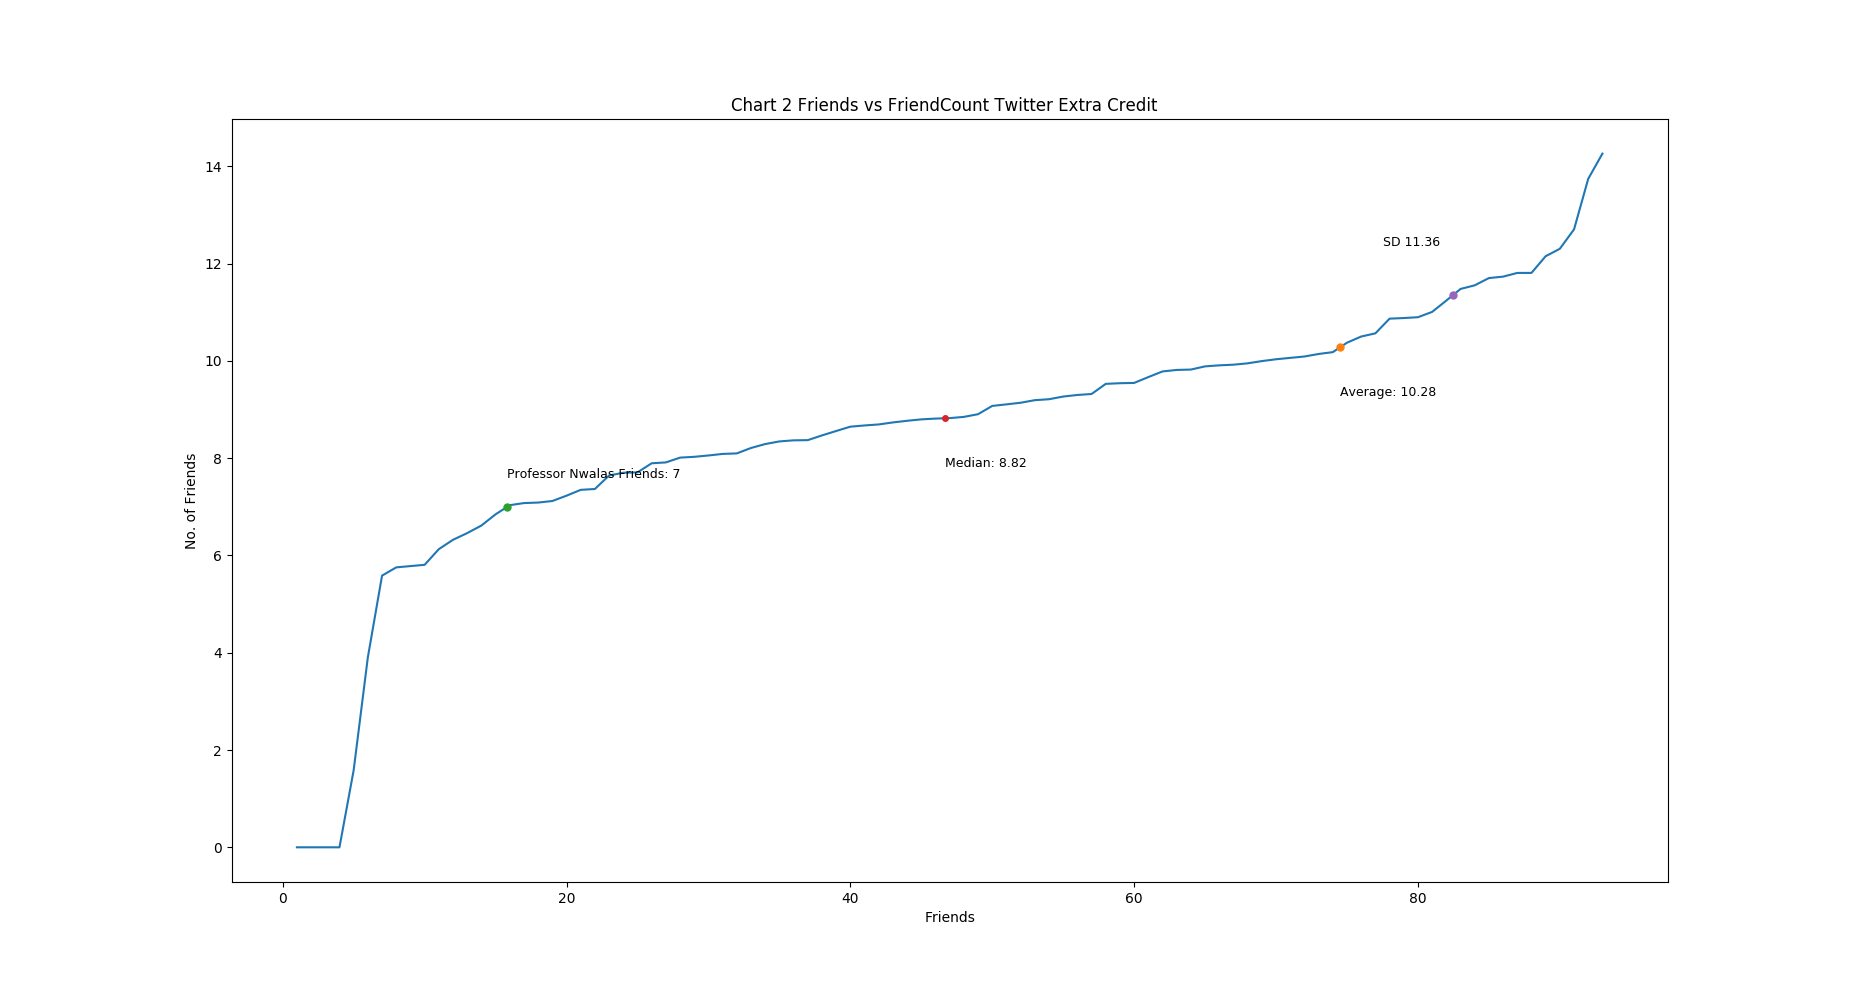
\includegraphics[width=\linewidth]{../Figures/ExtraCredit.png}
    \caption{Extra Credit Graph}
\end{subfigure}
\end{center}
\end{figure}

\tabto{2.0cm} It is evident that the friendship paradox holds in this situation as well. This is true because professor Nwala once again stands a substantial amount below average, with regards to the friend count. This dictates that most of professor Nwalas friends have more friends than he does, and thus the friendship paradox holds.


\end{document}
